% !TEX TS-program = pdflatex
% !TEX encoding = UTF-8 Unicode
%% For double-blind review submission
\documentclass[acmsmall,screen]{acmart}\settopmatter{printfolios=true}
%% For single-blind review submission
%\documentclass[acmlarge,review]{acmart}\settopmatter{printfolios=true}
%% For final camera-ready submission
%\documentclass[acmlarge]{acmart}\settopmatter{}

%% Note: Authors migrating a paper from PACMPL format to traditional
%% SIGPLAN proceedings format should change 'acmlarge' to
%% 'sigplan,10pt'.


%% Some recommended packages.
\usepackage{booktabs}   %% For formal tables:
                        %% http://ctan.org/pkg/booktabs
\usepackage{subcaption} %% For complex figures with subfigures/subcaptions
                        %% http://ctan.org/pkg/subcaption


\makeatletter\if@ACM@journal\makeatother
%\acmDOI{10.1145/nnnnnnn.nnnnnnn}
\startPage{1}
\else\makeatother
%% Conference information (used by SIGPLAN proceedings format)
%% Supplied to authors by publisher for camera-ready submission
%\acmDOI{10.1145/nnnnnnn.nnnnnnn}
\startPage{1}
\fi


%% Copyright information
%% Supplied to authors (based on authors' rights management selection;
%% see authors.acm.org) by publisher for camera-ready submission

%% Bibliography style
\bibliographystyle{ACM-Reference-Format}
%% Citation style
%% Note: author/year citations are required for papers published as an
%% issue of PACMPL.
\citestyle{acmauthoryear}   %% For author/year citations

\usepackage{uri}
\usepackage{mathtools}
\usepackage{amsthm}
\usepackage{mathpartir}
\usepackage{semantic}
\usepackage{graphicx}
\usepackage{cases}
\usepackage{hyperref}
\usepackage{stmaryrd}
\usepackage{listings}
\usepackage{iris}
%\usepackage{lstlangcoq}
\usepackage[edges]{forest}
\renewcommand{\lstlistingname}{Figure}

\clubpenalty = 10000
\widowpenalty = 10000
\displaywidowpenalty = 10000

\lstset{language=C,basicstyle=\ttfamily,mathescape=true,columns=fullflexible}

\newcommand{\TODO}[1]{\textbf{\textcolor{red}{[ TODO: #1]}}}
%\newcommand{\boxdotright}{\!\mathrel\boxdot\joinrel\rightarrow\!}
\newcommand{\islock}{\boxdotright}
\newcommand{\isaex}{\!\mathrel\odot\joinrel\rightarrow\!}
\newcommand{\xisaex}[1]{\!\mathrel\odot\joinrel\xrightarrow{#1}\!}
%% \newcommand{\ifthenelse}[3]{\text{if }#1\text{ then }#2\text{ else }#3}
\newcommand{\emp}{\mathsf{emp}}

\newcommand\dboxed[1]{\dbox{\ensuremath{#1}}}
\newcommand{\master}[2]{\ensuremath{\mathrm{Master}_{#1}(#2)}}
\newcommand{\snap}[1]{\ensuremath{\mathrm{Snapshot}(#1)}}
\newcommand{\ghost}[2]{\ensuremath{\dboxed{#1}^{#2}}}
\newcommand{\us}{$\mu$s}
\newcommand{\gnamety}{\ensuremath{\mathsf{gname}}}
\newcommand{\treerep}{\ensuremath{\mathsf{bst}}}
\newcommand{\nodeboxrep}{\ensuremath{\mathsf{bst\_ref}}}

\newcommand{\myhalf}[2]{\ensuremath{\mathsf{my\_half}_{#1}(#2)}}
\newcommand{\publichalf}[1]{\ensuremath{\mathsf{public\_half}(#1)}}

\newcommand{\ignore}[1]{}

\hyphenation{Comp-Cert}

\usepackage[utf8]{inputenc}
\usepackage{geometry}
\geometry{a4paper}

\usepackage{graphicx} % support the \includegraphics command and options
\usepackage{verbatim} % adds environment for commenting out blocks of text & for better verbatim
%\usepackage{amssymb}
\usepackage{url}
\usepackage{listings}

\title{Verifying Fine-Grained and Lock-Free Binary Search Trees}
\author{Roshan Sharma}
\author{Shengyi Wang}
\author{Alexander Oey}
\author{Anastasiia Evdokimova}
\author{Lennart Beringer}
\author{William Mansky}

\date{} % Activate to display a given date or no date (if empty),
         % otherwise the current date is printed 

\begin{document}
\acmConference{Some conference}
\maketitle

\catcode`\@=11
\section{Introduction}
The binary search tree (BST) is a common implementation of an ordered
map, a widely used data structure. The concurrent version of the
ordered map forms the bedrock of many parallel programs. We formally
verified the functional correctness of two versions of fine-grained
concurrent binary search trees (CBST) written in C. One adopts the
hand-over-hand locking technique \cite{bayer1977}, the other is lock
free by using atomic primitives such as compare and swap (CAS). Both
CBST implementations support insert, lookup, and delete operations; %or do we have lock-free without delete?
they also share the ``same'' specifications to some extent in our
verification. All the proof is machine-checked in Coq. %Say something about existing proofs of fine-grained data structures and how we compare.

Our specifications use the logical atomicity introduced in the TaDA
logic \cite{tada}, in the form of \emph{atomic Hoare
triples}. Intuitively, an atomic Hoare triple $ \langle
P \rangle\,\mathbb{C}\, \langle Q \rangle$ means the program
$\mathbb{C}$ ``atomically updates'' from $P$ to $Q$. The program may
actually take multiple steps, but every step before the atomic update
(linearization point) must preserve the assertion $P$. Meanwhile, the
concurrent environment may also update the state before the
linearization point, as long as the states satisfies $P$. The
assertion $Q$ must become true at the linearization point, then the
environment can do whatever it likes. There is no guarantee that $Q$
is still preserved when $\mathbb{C}$ returns. For example, the
specification of our \texttt{insert} operation may be explained as
follows: during the execution of \texttt{insert}, there is
always \emph{some} BST, and at some point the \texttt{insert} will
take a BST $t$, insert a value with a certain key, and then eventually
returns (meanwhile other threads may have further modified the
inserted tree)\footnote{Maybe say what a reasonable $Q$ is and why such a spec is still useful, specifically w.r.t. the situation where one of the other threads' action following the linearization point removes the element just inserted.}.

We employ the Verified Software Toolchain (VST) \cite{plfcc} to verify
the correctness of CBST. Although the concurrent separation logic
(CSL) has been formalized in VST rooted on the work of Hobor et
al.\ \cite{oraclesematic}, we extend it with two descendants of CSL so
as to accomplish the verification. One is the logical atomicity
mentioned above; the other is the higher-order ghost state in the
style of Iris \cite{higherorderghoststate}. The ghost states are used
to contruct both the global invariants and the local state in our
proofs. They will be further discussed in \S\ref{correctness}.

We highlight a few innovative aspects of our verification of CBST:
\begin{description}
\item [Range ghost] We abstract the BST via a pair of values
called \emph{range} which represents the lower-bound and upper-bound
of keys on each node to reason about the BST in the current
settings. We prove that range with the merging operation forms a
partial commutative monoid (PCM) so that it can be encoded in ghost
states.

\item [\textsf{sync\_inv} pattern] It is a particular approach
combining locks with general invariants to solve the dilemma caused by
the fine-grained locking mechanism: we do not have a lock to control
the access of the entire BST nor can we access the state of the BST
via atomic operations.
\end{description}

%% Do we have contributions, and are they sufficient? Range ghost is adapted from flow interfaces. Sync_inv pattern isn't totally ours, though it might be instructive w.r.t. combining traditional and Iris-style CSLs, and it might be worth explaining in more detail. We're working on "actual" code, but missing a few pieces to make our proofs foundational. (but maybe it's worth highlighting the extra work we do to work on actual code) We could promote this as the first working example of Iris+VST. We don't yet have any demonstrations on larger or interesting data structures, and this alone was quite a bit of work. The delete logic is rather interesting. Nothing to say about flow interfaces yet, but maybe soon.


Our specific contributions are:
\begin{itemize}
\item To the best of our knowledge, this is the first mechanized
verification of an concurrent search-based data structure written in a
real programming language. %should probably clarify what we mean by "real"

\item We illustrate how to incorporate the CSL in VST, the higher-order
ghost state in the style of Iris, and the logical atomicity from the
TaDA logic together to verify the CBST.
\end{itemize}

We introduce the background about the verification of concurrent C
programs in \S\ref{background}, including the tool-chain VST and Iris,
the concept of ghost states, global invariants, and atomic
specifications. The thread-safety proofs of operations on CBST are
first explained in \S\ref{safety}, where we show the \emph{recursive}
lock pattern for hand-over-hand locking mechanism. The functional
correctness proofs are presented in \S\ref{correctness}. We detail the
use of the \textsf{sync\_inv} pattern, the combination of recursive
lock invariants and ghost states together in the atomic
specifications, and the proof skeleton of each operation on CBST. The
related work is discussed in \S\ref{related}. We end with the
conclusion of our work in \S\ref{conclusion}.



\section{Background}
\label{background}
\subsection{VST and Iris}
We use the Verified Software Toolchain \cite{plfcc}  to prove the correctness of the concurrent binary search tree. VST is a Coq-based proof system that helps to prove separation logic properties of C programs with the assurance that the properties will be preserved in compiled code. First, we write programs in C programming and using CompCert’s \emph{clightgen}, the ASTs for C programs can be generated in Coq. We then state and prove specifications for them using Verifiable C. Verifiable C is a higher-order separation logic for reasoning about the functional correctness of C programs and carries a soundness proof that links high-level specifications to assembly code generated by the CompCert Verified compiler. Verifiable C supports reasoning about two separate kinds of concurrency:  Pthreads-style concurrency with locks (used by implementing blocking data structures that can be fine-grained or coarse-grained ), and concurrency using C11 atomic operations (i.e. lock-free data structures). 

\subsection{Ghost State and Global Invariants}
We can prove memory safety and race freedom properties of shared-memory concurrent programs, by tracking the transfer of ownership of shared locations between threads that would happen if we ran the program. But, this idea is insufficient to prove that concurrently running threads are successful to accomplish some task, which is also called functional correctness. For instance, we can prove the memory safety properties of the increment example in  \ref{figure1} through the transfer of ownership of shared variable $x$ between threads. But, we can not guarantee that the value of $x$ will be $2$ after all threads complete their execution, which is demonstrated in \ref{figure1} using separation logic assertion.   
\begin{figure}[htb]
\centering
$\texttt{x = 0;}$\\
$\mathit{I_{\pi}(x \mapsto v \land v \geq 0)}\qquad\pi = \pi_1\ .\ \pi_2$\\
$\begin{array}{l || l}
\mathit{I_{\pi_1}(x \mapsto v \land v \geq 0)} & \mathit{I_{\pi_2}(x \mapsto v \land v \geq 0)}\\
\texttt{acquire(l);} & \texttt{acquire(l);}\\
\mathit{x \mapsto v \land I_{\pi_1}(x \mapsto v \land v \geq 0)} & \mathit{x \mapsto v \land I_{\pi_2}(x \mapsto v \land v \geq 0)}\\
\texttt{x++;} & \texttt{x++;}\\
\mathit{x \mapsto v+1 \land I_{\pi_1}(x \mapsto v \land v \geq 0)} & \mathit{x \mapsto v+1 \land I_{\pi_2}(x \mapsto v \land v \geq 0)}\\
\texttt{release(l);} & \texttt{release(l);}\\
\mathit{I_{\pi_1}(x \mapsto v \land v \geq 0)} & \mathit{I_{\pi_2}(x \mapsto v \land v \geq 0)}\\
\end{array}$\\
$\mathit{I_{\pi}(x \mapsto v \land v \geq 0)}$
\caption{The increment example annotated with separation logic assertion}
\label{figure1}
\end{figure}
We must preserve the connection between the value of shared resources and the work performed by each thread. A common approach to achieve this is to use \emph{ghost variables}, an auxiliary state introduced later in the proof to track the local information about each thread. They do not appear in the original program. Program in \ref{figure1} can be verified by creating ghost state, which tracks the latest action performed by a thread, for each thread with initial value of $0$, and update with $1$ after each thread increment the value of \texttt{x}. In VST, we can create \emph{ghost state} for any Coq type in the form of an arbitrary \emph{partial commutative monoid} (PCM), a set with a partially defined binary operation that is as associative as it can, commutative, and has a unit, as long as we can describe what happens when two elements of that type are joined together. VST provides $\mathsf {ghost\_var}$ assertion to create a simple ghost state: $\mathsf{ghost\_var}\ \mathit{sh}\ a\ g$ asserts that $g$ is a \emph{ghost name} ($\gnamety$ in Coq) associated with the value $a$, which may be of any type. We will see different kind of ghost states used to verify binary search tree in the following sections.

The main idea behind the logic from Iris \cite{higherorderghoststate}, a mechnized higher-order concurrent separation logic framework, is the construction of \emph{global invariant} as \emph{ghost state}. \emph{Global Invariant} is an invariant on the global (ghost and physical) state of program. We can open any invariant but must close it again before taking any steps of execution unless those execution are atomic. Thread can use the contents of \emph{global invariant} during atomic operation if it can guarantee that no one will ever see an intermediate state in which invariant does not hold. The rules from Jung et al.\cite{higherorderghoststate} for creating and opening invariants are:

\begin{mathpar}
\inference[\textsf{inv\_alloc}]{}{\triangleright P \vdash \pvs[E] \mathsf{EX}\ i : \mathsf{iname}, \knowInv{i}{P}}

\inference[\textsf{inv\_open}]{i \in E}{\knowInv{i}{P} \vdash \pvs[E][E \setminus i] \triangleright P * (\triangleright P \wand \pvs[E \setminus i][E] \mathsf{emp})}
\end{mathpar}

where invariants are provided in the form of assertion $\knowInv{i}{P}$, and states that $P$ is maintained as an invariant on the global state with name $i$. The operator%%  $\pvs[][]$
is called ``fancy update" operator,that allows to allocate, open, and close the invariants and the later $\triangleright$ operator is used for impredicativity (i.e. $\knowInv{i}{..\knowInv{i}{P}..}$).

\subsection{Atomic Specifications}
\label{atomic}
For many concurrent data structures, the ideal correctness condition is that the data structure behaves the same as a sequential implementation, even when accessed simultaneously by multiple threads. This intuitive condition can be formalized as linearizability (operations appear to take effect in some total order) or atomicity (client threads never observe intermediate states of operations). In separation logic, atomicity can be expressed in the form of \emph{atomic triples}~\cite{tada}, written in the form $\forall a.\ \langle P_l\ |\ P_p(a)\rangle\ c\ \langle Q_l\ |\ Q_p(a)\rangle$, where $P_l$ and $Q_l$ are \emph{private} pre- and postconditions similar to an ordinary Hoare triple, and $P_p$ and $Q_p$ are \emph{public} pre- and postconditions, parameterized by an abstract value $a$ of the shared data structure. Intuitively, $P_l$ and $Q_l$ must be true before and after the call, while $P_p$ must be true for some value of $a$ at every point from the beginning of $c$ until some designated linearization point, at which point $Q_p$ becomes true atomically for the same value $a$. For instance, the specification $$\forall s.\ \langle \mathsf{is\_stack}\ p\ |\ \mathsf{stack}\ s\rangle\ \texttt{push}(v)\ \langle \mathsf{is\_stack}\ p\ |\ \mathsf{stack}\ (v :: s)\rangle$$ expresses the fact that the \texttt{push} operation of a concurrent stack correctly implements the behavior of a sequential push, atomically transitioning from some stack $s$ to $v :: s$ at some point during its execution. %maybe something about linking ghost state, which parts are real vs. ghost, accessing invariants around atomic triple

VST has encoded an atomic Hoare triple, and provide the way that matches the notation VST uses for normal specifications. Such specification is called \emph{atomic specification}, and can be formalized in Coq as shown in  \ref{atomic-spec}.  This is how we write pre- and postcondition in VST. 
\begin{figure}[htb]
\centering
\begin{verbatim}
Program Definition insert_spec :=
DECLARE _insert
ATOMIC TYPE W OBJ a INVS Ei Eo
WITH ...
PRE [ ... ]
  PROP (...)
  LOCAL (...)
  SEP (P_l) | (P_p)
POST [ ... ]
  PROP ()
  LOCAL ()
  SEP (Q_l) | (Q_p)
\end{verbatim}
\caption{Atomic Specification in VST}
\label{atomic-spec}
\end{figure}
\texttt{W} is the \textsf{TypeTree} representing the type of arguments passed with \texttt{WITH} clause; \texttt{a} is the abstract state for the triple; \texttt{Ei} and \texttt{Eo} are the sets of invariants names inside and outside the triple. The \texttt{PROP} clause describes things that that are true independent of program state, the \texttt{LOCAL} clause describes the values contained in C local variables, and the \texttt{SEP} clause represents the \emph{separating conjunction} (*) of \emph{spatial predicates}, predicates on some part of the memory. In VST, while proving that a function implements an atomic specification, the precondition will contains an $\mathsf{atomic\_shift}$ assertion with the public pre- and postcondition, and the masks inside it. This atomic shift can be accessed through following two rules:
$$\inference[\textsf{atomic\_commit}]{\forall a, R * P_p\ a \Rrightarrow \mathsf{EX}\ y,\ Q_p\ a\ y * R'\ y}{\textsf{atomic\_shift}(P_p, E_i, E_o, Q_p, Q) * R \Rrightarrow \mathsf{EX}\ y,\ Q\ y * R'\ y}$$
$$\inference[\textsf{atomic\_rollback}]{\forall a, R * P_p\ a \Rrightarrow P_p\ a * R'}{\textsf{atomic\_shift}(P_p, E_i, E_o, Q_p, Q) * R \Rrightarrow \textsf{atomic\_shift}(P_p, E_i, E_o, Q_p, Q) * R'}$$
During commit, we must provide resources $R$ which, in combination with the public precondition $P_p$, allow us to prove the public postcondition $Q_p$. Then, we gain access to an assertion $Q$ required by the postcondition of the function, and leftover resources $R'$. During rollback, we provide resources $R$ which, in combination with the public precondition, allow us to reestablish the public precondition; we then regain the atomic shift back in the proof, as well as leftover resources $R'$. The rollback is specially used to learn some relationship between pieces of information (e.g. ghost state) stored in the public precondition, while the commit is used to prove the public postcondition from the precondition, and obtain an assertion $Q$. To complete the proof of any function's specification, we must always perform commit to obtain $Q$; we can perform any number of roolbacks before that point, but after that point we lose the atomic shift and no access to the public precondition.

\ignore{\section{Safety Proofs} %maybe cut this, or roll it into the next section
\label{safety}
\begin{figure}[htp]
\begin{subfigure}[t]{\textwidth}
\begin{lstlisting}[language = C]
typedef struct tree {int key; void *value; struct tree_t *left, *right;} tree;
typedef struct tree_t {tree *t; lock_t *lock;} tree_t;
typedef struct tree_t **treebox;

void insert (treebox t, int x, void *value) {
  struct tree_t *tgt = *t;
  struct tree *p;
  void *l = tgt>lock;
  acquire(l);
  for(;;) {
    p = tgt->t;
    if (p==NULL) {
      tree_t *p1 = (struct tree_t *) surely_malloc (sizeof *tgt);
      tree_t *p2 = (struct tree_t *) surely_malloc (sizeof *tgt);
      p1 ->t = NULL;
      p2 ->t = NULL;
      lock_t *l1 = (lock_t *) surely_malloc(sizeof(lock_t));
      makelock(l1);
      p1->lock = l1;
      release2(l1);
      lock_t *l2 = (lock_t *) surely_malloc(sizeof(lock_t));
      makelock(l2);
      p2->lock = l2;
      release2(l2);
      p = (struct tree *) surely_malloc (sizeof *p);
      tgt->t = p;
      p->key=x; p->value=value; p->left=p1; p->right=p2;
      release2(l);
      return;
    } else {
      int y = p->key;
      if (x<y){
      	tgt = p->left;
        void *l_old = l;
        l = tgt->lock;
        acquire(l);
        release2(l_old);
      } else if (y<x){
        tgt = p->right;
        void *l_old = l;
        l = tgt->lock;
        acquire(l);
        release2(l_old);
      }else {
      	p->value=value;
        release2(l);
      	return;
      }
    }
  }
} 
\end{lstlisting} 
\end{subfigure}
\caption{Insert Method}
\label{insert}
\end{figure}     
\begin{figure}[htp]
\begin{subfigure}[t]{\textwidth}
 \begin{lstlisting}
void *lookup (treebox t, int x) {
  struct tree *p; void *v;
  struct tree_t *tgt;
  tgt = *t;
  void *l = tgt->lock;
  acquire(l);
  p = tgt->t;
  while (p!=NULL) {
    int y = p->key;
    if (x<y){
      tgt=p->left;
      void *l_old = l;
      l = tgt->lock;
      acquire(l);
      p=tgt->t;
      release2(l_old);
    }else if (y<x){
      tgt=p->right;
      void *l_old = l;
      l = tgt->lock;
      acquire(l);
      p=tgt->t;
      release2(l_old);
    }else {
      v = p->value;
      release2(l);
      return v;
    }
  }
  release2(l);
  return NULL;
}
\end{lstlisting}
\end{subfigure}
\caption{Lookup Method}
\label{lookup}
\end{figure}
In this section, we will focus on safety proofs of concurrent binary search tree. Here safety means thread-safe. An operation of any concurrent data-structure is thread-safe if it functions correctly during simultaneous execution by multiple threads. A thread can update the data structure if it holds a sufficiently large share of the data structure so that no other thread can possibly read it. If we want to have a data structure that can be modified by multiple threads, we must move shares between threads via locks. In VST, we can use $\mathsf{lock\_inv}$ assertion to assert that there exists a lock in memory with a given invariant: $\mathsf{lock\_inv}\ \mathsf{sh}\ p\ R$ means that the current thread owns share $\mathsf{sh}$ of a lock at location $p$ with invariant $R$. We use the term \emph{lock invariant} for $R$, which is a predicate representing the resources protected by a lock. The $\mathsf{lock\_inv}$ predicate is sufficient to prove the safety properties of the concurrent data-structure. 

%We have taken binary search tree with fine-grained locking. In hand-over-hand locking mechanism, we acquire the lock for a successor before releasing the lock for a predecessor. The code for $\texttt{insert}$ and $\texttt{lookup}$ methods of concurrent binary search tree that we are interested to verify is presented in Figure 1. 
   
\subsection{Lock invariants for hand-over-hand locking}
A node of CBST have the pointer to its children, so lock invariant of a node should have the knowledge about its children.   
Whenever we release the lock for the parent node, we have to recover all resources that the parent node accessed while acquiring the lock. By releasing the parent node's lock, we would lose the information about the lock\_inv of the node and we would not be able to release the node's lock later. To solve this problem, we use \emph{recursive} lock, one whose invariant includes a share of lock itself so that we can retain lock\_inv assertion for a node even after releasing its parent's lock. In VST, we can make such an invariant using $\mathsf{selflock}$ function along with the lemma $\mathsf{selflock\_eq}$: $\forall Q\ \mathit{sh}\ p, \mathsf{selflock}\ Q\ \mathit{sh}\ p = Q * \mathsf{lock\_inv}\ \mathit{sh}\ p\ (\mathsf{selflock}\ Q\ \mathit{sh}\ p)$. We can define $\mathsf{lock\_inv}$ predicate for \emph{recursive} lock $\mathit{lock}$ as follows: $\mathsf{lock\_inv}\ \mathit{sh1}\ p\ (\mathsf{selflock}\ P\ \mathit{sh2}\ \mathit{lock})$ where $\mathit{P}$ represents the knowledge about the children of current node, $\mathit{sh1}$ and $\mathit{sh2}$ are the two halves of the writable share.

\subsection{Specification and Verification}
We begin the verification by defining a predicate $\nodeboxrep(p)$ that describes the concrete representation of the tree, where $p$ is the pointer to the root node. The $\texttt{nodebox\_rep}$ predicate ties together $\texttt{lock\_inv}$ assertion for each recursive lock as follows: 
\begin{align*}
 &\nodeboxrep_{\pi}(p) \triangleq  p\mapsto\ (lock,tp)\ *\ \mathsf{lock\_inv_{\pi}}(lock, \mathsf{selflock}_{0.5}(lock,R))) \\&R  \triangleq\ \exists\ pa\ pb\ \ tp\mapsto\ (pa * pb)\ *\  \nodeboxrep_{0.5}(pa)\ *\ \nodeboxrep_{0.5}(pb)  \end{align*}
 
 The ownership of each node's lock is divided into two halves: one half is owned by \emph{lock\ invariant} and another half is owned by node itself. But, in case of root node, we need to split one half into multiple pieces, and share those pieces to all threads such that all of them initially have the knowledge of root node.
 
 The \emph{lock}, used in the implementation of BST operations, provides \texttt{acquire} and \texttt{release} functions, which allow threads to transfer ownership of resource invariants. Their pre- and postconditions are as follows:
$$\{!!\mathsf{readable\_share}\ \mathit{sh} \land \mathsf{lock\_inv}\ \mathit{sh}\ \ell\ R\}\ \texttt{acquire}(\ell)\ \{R * \mathsf{lock\_inv}\ \mathit{sh}\ \ell\ R\}$$
$$\{!!(\mathsf{readable\_share}\ \mathit{sh} \land \mathsf{exclusive}\ R) * R * \mathsf{lock\_inv}\ \mathit{sh}\ \ell\ R\}\ \texttt{release}(\ell)\ \{\mathsf{lock\_inv}\ \mathit{sh}\ \ell\ R\}$$


The resource invariant $R$ need to be \emph{exclusive}, i.e, it can only hold once in any given state. This allows us to know that if the current thread holds the invariants, it also hold the lock. 
}
    
\section{BST with Hand-over-Hand Locking}
\label{hand-over-hand}
As described in section~\ref{atomic}, we want the operations of our concurrent BSTs to satisfy atomic triples relating them to sequential operations:
\begin{mathpar}
\forall t.\ \langle \nodeboxrep\ p\ |\ \treerep\ t\rangle\ \texttt{insert}(p, k, v)\ \langle \nodeboxrep\ p\ |\ \treerep\ (\mathrm{insert}\ t\ k\ v)\rangle

\forall t.\ \langle \nodeboxrep\ p\ |\ \treerep\ t\rangle\ \texttt{lookup}(p, k)\ \langle v.\ \nodeboxrep\ p\ |\ \treerep\ t \land \mathrm{lookup}\ t\ k = v\rangle

\forall t.\ \langle \nodeboxrep\ p\ |\ \treerep\ t\rangle\ \texttt{delete}(p, k)\ \langle \nodeboxrep\ p\ |\ \treerep\ (\mathrm{delete}\ t\ k)\rangle
\end{mathpar}
In our case, insert, lookup, and delete are simple Gallina functions on a functional tree data structure. The details of $\nodeboxrep$ and $\treerep$ may vary by implementation, but we expect that $\nodeboxrep$ contains at least a pointer to the data structure, and $\treerep$ contains some ghost state linking the concrete state of the data structure to the abstract tree $t$.

In the following sections, we describe the construction of these predicates, and the proofs of the operations, for BST implementations based on hand-over-hand locking and lock-free atomic operations.

%look at some of the Iris papers in CPP, etc. for how we should describe the proofs, e.g. section 4 of Formal Verification of a Concurrent Bounded Queue in a Weak Memory Model, Mevel and Jourdan, ICFP 2021

%%%%%%%%%%%%%%%%%%%%%

\ignore{In the previous section, we showed that how to prove concurrent data-structure is thread safe, but not functionally correct. To prove the correctness, our threads need to be able to record the information about the actions they have performed on the shared state, instead of sealing all knowledge of the shared data structure inside the lock invariant. We can accomplish this with ghost variables, a simple form of auxiliary state. Aside from the \emph{permission} on shared resources held by each thread that we used in the safety proofs, the verification of correctness properties also involves the \emph{ghost state}. In VST, any Coq type can be used as ghost state, as long as we can describe what happens when two elements of that type are joined together. We can use own predicate in VST to represent ghost state assertion as follows: $\mathsf{own}\ g\ a\ \mathit{pp}$, where $g$ is a \emph{ghost name}, $a$ is the value associated with $g$ which can be of any type, and $\mathit{pp}$ is a separation logic predicate.}


%Linearizability is one of the most popular strong correctness condition for the most of %concurrent data-structure, which implies that every operation appears to take place atomically, %in some order, consistent with the real-time ordering of those operations. 
%In order to record the action each thread performed as a linear history, we will define global %invariants using the ghost state, which are similar to lock invariants but are not associated %with any particular memory location. Instead, a global invariant is true before and after every %step of a program, acting as a publicly accessible resource. A program instruction can use the %contents of global invariant if it can guarantee that no one will ever see an intermediate state %in which the invariant does not hold. 

\subsection{Fine-grained locking and atomicity}
\label{atomicity}

To prove that an operation on a data structure satisfies a logically atomic specification, we must show that there are no visible intermediate states of the operation, i.e., that other threads see the data structure as unchanged until the linearization point at which the operation takes effect. In traditional concurrent separation logics such as VST's~\cite{oraclesematic}, this is done by protecting the data structure with a single lock whose \emph{lock invariant} describes consistent states of the data structure. In modern separation logics such as Iris~\cite{iris} or FCSL~\cite{fcsl}, we can make a series of atomic modifications to the data structure without continuously holding a lock, as long as one modification can be designated the \emph{linearization point} at which the new state becomes public, and all prior changes are invisible to other threads. Fine-grained locking, in which the pieces of a data structure are each protected by a separate lock with a traditional lock invariant, requires us to synthesize these two approaches: we may make a series of non-atomic modifications to a part of the data structure as long as we hold its lock, but when we release the lock we need to ensure that either we have reached the linearization point, or our changes are invisible to other threads.

We accomplish this using a technique derived from unpublished work by Jung~\cite{ralf-convo} for treating the critical sections of locks as atomic operations. The key is to include in each lock invariant a piece of ghost state that represents the abstract state of the locked section. From the outside, the effect of the critical section is to atomically update that piece of ghost state, and all other changes are internal to the lock. These pieces of ghost state can then be composed to yield the abstract state of the entire data structure. In effect, this construction turns a traditional lock invariant into a \emph{lock variant} $\ell \islock R(a)$, where the value of $a$ can be updated in the critical section as long as it corresponds to a linearization point or invisible change to the abstract state of the data structure as a whole. This allows traditional lock invariants to interact with atomic shifts and be used to prove atomic specifications.

The construction of the lock variants is simple. We begin with a \emph{part-reference} ghost state, a common construction for sharing information between an invariant and the threads that act on it, with elements $\publichalf{a}$ (the current state $a$) and $\myhalf{\pi}{p}$ (partial information about the current state, annotated with a share $\pi$). When the share $\pi$ is 1, we know that $p = a$. (do we want to define this ourselves, or reference it somewhere? note also that this is what Iris calls an authoritative algebra) A lock variant with an assertion $R(a)$ is then defined as %notation
$$\ell \islock R(a) \triangleq \ell \islock \exists a.\ R(a) * \myhalf{\pi}{a}$$ %eliding ghost names here
The share $\pi$ may be set to 1 if the lock's information about $a$ is always fully up to date, or a smaller share if it can become outdated due to operations on other parts of the data structure. Since $a$ is existentially quantified, a thread that changes the value of $a$ forgets it after releasing the lock (as required in a lock invariant), but it must have synchronized with a $\publichalf{a}$ held elsewhere (usually in a global invariant) that will remember the change. Thus, the ghost state acts as a bridge between the component lock invariant and the global abstract state of the data structure. %smaller example before we get into BST?

From the atomic rules of section~\ref{atomic}, we derive the following rules for accessing and modifying pieces of the global abstract state:
\begin{mathpar}
\inference[\textsf{sync\_commit}]{\forall a.\ R * P_p\ a \Rrightarrow \exists x_1.\ \mathsf{public\_half}(g, x_1) * \exists x_0',\,x_1'.\ (x_0, x_1) \leadsto (x_0', x_1')\ \land \\(\mathsf{my\_half}(g, \mathit{sh}, x_0') * \mathsf{public\_half}(g, x_1') \Rrightarrow \exists y.\ Q_p\ a\ y * R'\ y)}{\textsf{atomic\_shift}(P_p, E_i, E_o, Q_p, Q) * \textsf{my\_half}(g,sh,x_0) * R \Rrightarrow \mathsf{EX}\ y,\ Q\ y * R'\ y}

\inference[\textsf{sync\_rollback}]{\forall a.\ R * P_p\ a \Rrightarrow \exists x_1.\ \mathsf{public\_half}(g, x_1) * (\mathsf{public\_half}(g, x_1) \Rrightarrow P_p\ a * R')}{\begin{array}{c}\textsf{atomic\_shift}(P_p, E_i, E_o, Q_p, Q) * \textsf{my\_half}(g,sh,x_0) * R  \Rrightarrow \\\textsf{atomic\_shift}(P_p, E_i, E_o, Q_p, Q) * \textsf{my\_half}(g,sh,x_0) * R'\end{array}}
\end{mathpar}
A thread that holds $\myhalf{}{a}$ (i.e., is in the critical section of a lock with a lock variant) may interact with the abstract state $P_p$ held in an $\textsf{atomic\_shift}$, as long as the corresponding $\publichalf{}$ is part of the abstract state. It may either leave both halves as is and gain updated resources $R'$ (including, e.g., a snapshot of the current abstract state), or update both halves to a new state that satisfies the public postcondition $Q_p$, executing the linearization point and obtaining the final postcondition $Q$. Typically we will use one of these rules at the end of each critical section, to show that the changes made in the critical section either are invisible to other threads (\textsf{sync\_rollback}) or have fulfilled the linearization point (\textsf{sync\_commit}). We can also derive simpler rules for special cases, such as a version of \textsf{sync\_commit} for read-only operations that do not change the state of any component:

$$\inference[\textsf{sync\_commit\_same}]{\forall a.\ R * P_p\ a \Rrightarrow \exists x_1.\ \mathsf{public\_half}(g, x_1) * (\mathsf{my\_half}(g, \mathit{sh}, x_0) * \mathsf{public\_half}(g, x_1) \Rrightarrow \exists y.\ Q_p\ a\ y * R'\ y)}{\textsf{atomic\_shift}(P_p, E_i, E_o, Q_p, Q) * \textsf{my\_half}(g,sh,x_0) * R \Rrightarrow \mathsf{EX}\ y,\ Q\ y * R'\ y}$$

\subsection{Specification of the hand-over-hand BST}
%rewrite to use the above: this is the global state made up of components, etc.

To verify our tree implementation, we need to instantiate $\nodeboxrep$ (the resources held by each client thread) and $\treerep$ (the abstract state of the data structure), and show how they interact to access and update the state of the data structure for each call. In a lock-based implementation, $\nodeboxrep$ will be a pointer to the lock of the root node, and acquiring that lock will give the thread access to more of the data structure. Our overall approach is to associate a piece of ghost state with each node in the tree, which will be shared between that node's lock and the abstract state in $\treerep$. We also need to make sure that our lock invariants support the hand-over-hand pattern.

\subsubsection{Ghost States and Range}
 The main challenge in proving the properties of concurrent data structure is to abstract the data structure in a way that helps to reason about it in the concurrent setting. Krishna et al. \cite{krishna2017flow} mention in their paper that we can abstract binary search tree using appropriate bounds in each node: we can use the product of \emph{lower-bound} and \emph{upper-bound} on each node of binary tree by propagating from each node to its child the appropriate bounds on the values presents in the sub-tree. The \emph{lower-bound} and \emph{upper-bound} help us to prove that we perform the operation in the right node: for instance, if we $\mathsf{insert}$ a key in the tree, then key should be inside those two bounds. We use the term \emph{range} to represent the product of lower- and upper-bound. \ref{range_bst} shows an example of BST with each node labeled with appropriate bound propagated all the way from \emph{root} to empty \emph{leaf} nodes. 
\begin{figure}[htb]
\centering
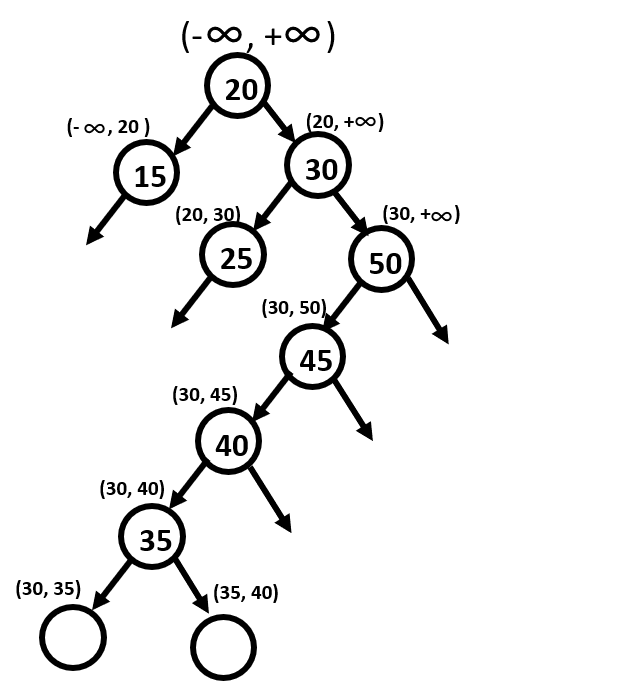
\includegraphics[width=70mm,scale=0.5]{FIG/range_prop.png}
\caption{An example of BST with each node labeled with \emph{range}; lower and upper bound for a key}
\label{range_bst}
\end{figure}
The range for root node is always $(-\infty,+\infty)$ and then, we can calculate the range for all nodes in the tree by enforcing each node to propagates appropriate bounds. For the left child, range will be lower-bound for the node (lower-bound) and the key in the node (upper-bound), while for the right child range will be a key in the node (lower-bound) and upper-bound for the node (upper-bound). This properties in each node help us to prove that the thread have changed the state of data-structure to the valid state. For instance, we can confirm that a key has been inserted in the right place if a key is inside the range of the node. Suppose we want to insert a key $38$ in \ref{range_bst}, then we will locate \emph{right} child of $35$ as the right place for $38$. During insertion, we can confirm that the node is indeed right place for $38$ by checking that $38$ is in the range (35,40). We introduce the $range$ in our proof using the ghost variables. This $ranges$ along with other information about the node represent the abstract state of the data structure. We have used two kind of ghost state in our proof: \emph{per-node} ghost state and \emph{overall} ghost state.\\
\textbf{Per-node Ghost State}: The per-node ghost state is includes a node's range and other information about the node: its current key, value, and ghost names of its child nodes. In VST, we can use a type as ghost state by proving an instance of the \texttt{Ghost} typeclass, analogous to the \emph{resource algebras} of Iris. The essential part is a \emph{join} relation describing how two pieces of ghost state combine. We define the join of two ranges to be the range that contains both of them, and use an \emph{exclusive} algebra for the rest of the data, so that only one thread knows the current state of a node at a time. 
Ghost state is shared between the per-node lock invariants and the abstract state of the data structure using the \emph{reference} pattern: each thread holds partial information describing its contribution to the shared state, and the shared resources hold a ``reference'' copy that records all of the contributions. In VST, this is implemented with assertions $\mathsf{my\_half}\ g\ \mathit{sh}\ a$ and $\mathsf{public\_half}\ g\ r$, where $g$ is the node's identifier ($\gnamety$), $a$/$r$ is the value of the ghost state, and $\mathit{sh}$ is a share describing how much of the reference value is known: if $\mathit{sh}$ is the full share, then we know that $a = r$. In the proof, the \texttt{my\_half} assertion for a node will be held by the node's lock, and \texttt{public\_half} will be held by the shared state.

\textbf{Overall Ghost State}: We now have per-node ghost state for each node, indexed by a ghost name $g_n$. But if we are given an arbitrary $\gnamety$ for a node, we do not know whether that $\gnamety$ exists in the tree. We need another kind of ghost state to hold the set of all nodes in the current tree. Again we can use the ``reference'' pattern to define this ghost state, where the abstract state $\mathsf{ghost\_ref}\ s$ holds the full set of nodes, and each node's lock invariant holds an $\mathsf{in\_tree\ g_n}$ assertion guaranteeing that $g_n$ is in $s$.%notation for gnames
\ignore{\begin{verbatim}
Definition ghost_ref g r1 := ghost_reference(P := set_PCM) r1 g.
Definition in_tree g g1 := EX sh: share, ghost_part(P :=set_PCM) sh (Ensembles.Singleton g1) g.
\end{verbatim}}
\ignore{The global invariant, which we introduced in our atomic specification as the $\treerep$ predicate above, ties together the pieces as follows:
\begin{align*}\treerep(T,g) \triangleq *_n. \mathsf{public\_half\textsubscript{gn}} \ (\mathit{range}_n* \mathit{ghost\_info}_n)\ ] *\ \mathsf{ghost\_ref}\ g\ \{ gn\  \} \end{align*}
 Later while writing atomic specification, we will use $\mathsf{ghost\_ref}$ and $\mathsf{in\_tree}$ in the public and private part respectively. Once we open \emph{global invariant}, we get access to $\mathsf{ghost\_ref}$ which will be used with $\mathsf{in\_tree}$ to establish the fact that node actually exists in the tree. We proved the following lemma for this:
$$
Lemma\ \mathbf{\ node\_exist\_in\_tree : }\ \forall\ g\ s\ g\_in,\  \mathbf{in\_tree}\ g\ g\_in  * \mathbf{ghost\_ref}\ g\ s\ \Rightarrow\ g\_in\ \in s .
$$}
\subsubsection{Handle and Abstract State}
Now we are ready to define the $\treerep$ and $\nodeboxrep$ predicates.

describe lock invariant

We combine pieces of information discussed above, \emph{recursive lock invariant} from \ref{safety} and \emph{ghost states}, to write the atomic specification. The private pre- and postcondition of the atomic specification is given by defining the predicate $\nodeboxrep(p,g,g\_root)$ that describes the concrete state of the BST along with the contribution part of the both kind of ghost states explained above.The root node $p$ is represented by ghost name $g\_root$ and overall ghost state is represented by ghost name $g$. The $\nodeboxrep$ predicate ties together $\mathsf{my\_half}$ part of per-node ghost state and $\mathsf{in\_tree}$ of over-all ghost state inside the $\mathsf{lock\_inv}$ assertion of each node's lock as follows:
\begin{align*}
    &\nodeboxrep_{\pi}(p,g,g\_root) \triangleq  p\mapsto\ (lock,tp)\ *\ \mathsf{lock\_inv_{\pi}}(lock, \mathsf{selflock}_{0.5}(lock,R))) \\&R  \triangleq\ \ghost{\mathsf{my\_half}(range,info)}{g\_root}\ *\ \ghost{\mathsf{in\_tree}\ (g\_root)}{g}\ *\ \exists\ pa\ pb\ ga\ gb,\ tp\mapsto\ (pa * pb)\ *\  \nodeboxrep_{0.5}(pa,g,ga) \\& *\ \nodeboxrep_{0.5}(pb,g,gb))\end{align*}
    
The public pre- and postcondition of the atomic specification is given by defining the predicate $\treerep(T,g)$ that describes the abstract state of the binary search tree $T$  in terms of collection of ghost states each describing the information about separate node in the tree.. The $\treerep$ predicate ties together $\mathsf{public\_half}$ part of per-node ghost states and $\mathsf{ghost\_ref}$ of over-all ghost state as follows: \begin{align*}&\mathsf{ghost\_tree\_rep}(tg,range, g, g\_current) \triangleq\ \exists\ k, v, ga, gb\ \in tg,\ghost{\mathsf{public\_half}\ (range, Some(k,v,ga,gb))}{g\_current}\\& *\ \mathsf{ghost\_tree\_rep}(left(tg),(left(range),k),g,ga)\ *\ \mathsf{ghost\_tree\_rep}(right(tg),(k, right(range)),g,gb) \end{align*}
\begin{align*}\treerep(T,g,g\_root) \triangleq \ \exists\ (tg:ghost\_tree),\ &\mathsf{pure\_tree}(tg)\ =\ T\ \land\ \mathsf{ghost\_tree\_rep}(tg,(-\infty, +\infty),g,g\_root)&\\ *\ \ghost{\mathsf{ghost\_ref}\ (\mathsf{find\_ghost\_set}(tg))}{g}\end{align*}
Where $tg$ is called \emph{ghost tree}, which can be existentially quantified, extend the node in pure tree $T$ with actual pointer and ghost names for child nodes. 

The atomic specification for any binary search tree's operation \texttt{op} should then be
\begin{align*}\forall t.\ \langle \nodeboxrep(p,g,g_{\mathit{root}})\ |\ \treerep(t,g)\rangle\ \texttt{op}(p)\ \langle \nodeboxrep(p,g,g_{\mathit{root}})\ |\ \treerep(t', g)\rangle
\end{align*}
where $t$ and $t'$ are the abstract state of a tree before and after the function's execution. Now we are prepared to prove that each of our BST functions satisfies its specification.

\subsection{Proofs: Insert and Lookup}
The basic verification style in VST is to divide proofs into two parts: proofs that the C implementations meet specifications that are Coq-level encodings of their behavior, and proofs that those encodings actually have the desired properties. In the single-threaded case, we might prove that some code implements a binary search tree written in Gallina, and then prove that that tree satisfies map axioms. Similarly, we divide our concurrency proofs into two parts: code-specific proofs that describe how the C code implements changes to per-node ghost state, and more abstract proofs describing how changes in local ghost state lead to the desired updates to the global state.

\subsubsection{Insert}
An outline of the C code for the insert function is shown in figure \ref{insert-proof}. When a thread inserts a key $k$ into a tree, it first crawls the tree to find the right position for $k$ using the hand-over-hand locking mechanism, acquiring the lock for the next node before releasing the lock for the current node. If it encounters a node with key $k$, then it simply changes the value at that node. Otherwise, it will eventually reach a leaf node, where it creates two new empty leaf nodes, inserts the key and value into the current node, and links the newly created leaf nodes to the current node. The atomic specification for insert method is $$\forall t.\ \langle \nodeboxrep\ p\ |\ \treerep\ t\rangle\ \texttt{insert}(p, k, v)\ \langle \nodeboxrep\ p\ |\ \treerep\ (\mathrm{insert}\ t\ k\ v)\rangle$$
The \texttt{insert} function should atomically add the key $k$ with value $v$ to the tree at $p$.

The key to the verification of the C code is the loop invariant for the top-level loop. We define the loop invariant for the insert function as follows: 
\begin{align*} &\mathsf{insert\_inv}(b, x, g, g\_root) \triangleq\ \exists\ \mathit{lock},\mathit{g\_current},\mathit{np},\mathit{range},\mathit{info},\ (x\in \mathit{range})\ \land \ \ghost{\mathsf{my\_half}(\mathit{range},\mathit{info})}{g\_current}\ *\ R\ \mathit{np}\\& * \mathsf{lock\_inv}(\mathit{lock},\mathit{lsh2},R')\ *\ \nodeboxrep(b,g,\mathit{g\_root})\ *\ \mathsf{atomic\_shift} (P_p,E_i,E_o,Q_p,Q) \end{align*}   
where $P_p$ and $Q_p$ are $\treerep(t,g)$ and $\treerep(t[k\mapsto v],g)$ respectively. The resources $R$, parameterized by a node pointer $\mathit{np}$, describes the concrete information about a node. Also, $x$ is the key to be inserted that must be in the bound $\mathsf{range}$.  This loop invariant has some existential variables which characterize the state of each iteration of the loop.

Figure \ref{insertproof} shows the $\texttt{insert}$ function with separation logic annotations. The proof starts with $\nodeboxrep$ and $\mathsf{atomic\_shift}$ as the precondition. After acquiring the lock for the root node, the thread accesses the information inside the lock invariant of the root node. In order to prove $\mathsf{while}$ loop, we show that the precondition satisfies the $\mathsf{insert\_inv}$, then prove that the loop body preserves the loop invariant (cases inside $\mathsf{else if}$ clauses at line 15 and 17 in \ref{insert}).   Once we locate the empty node for inserting the new key-value pair (inside the first $\mathsf{if}$ clause), we open the global invariant encoded in the $\mathsf{atomic\_shift}$, create the ghost names $\texttt{g1}$ and $\texttt{g2}$ for two new empty child nodes of current node, and use the $\mathsf{sync\_commit}$ rule---we have reached the linearization point and completed the insertion. The premise of $\mathsf{sync\_commit}$ requires that we have enough information to know that inserting the key at this point will change the abstract state from some unknown $t$ to $t[k\mapsto v]$, which we show in the second part of the proof.

The other branch of the code-level proof is the case where the key to be inserted already exists in the tree (the last $\texttt{else}$ clause in the code). %The modification of the global state of the tree t is shown in \ref{extract_insert2}. In that case, the old value $v'$ associated with key is overridden by new value $v$ keeping a key $40$ and child pointers as as they are. This is also the \emph{linearization point} of the $\mathsf{insert}$ operation. We augment the same $\emph{extract}$ lemma with the clause that states the scenario in \ref{extract_insert2}, and prove the lemma in the same induction over the tree $t$.
In this case, we change the value at the node but leave the rest of the tree intact, and this is the linearization point for the insertion. In the second part of the proof, we will show that this case also transforms $t$ to $t[k\mapsto v]$.

In the other two cases, we compare the key
of the current node with the new key \texttt{x} and move to the left or right child accordingly. Here we again need to access the atomic shift, to ensure that the range of the node we move to is included in the range of the current node. We can use $\mathsf{sync\_rollback}$ to retrieve this information without making any changes to the abstract state of the tree. %For the left branch case, we accomplish the proof by the following lemma:
%\begin{verbatim}
%Lemma in_tree_left_range:
%  forall (B: Type) (b: tree -> B -> mpred) (Q : B → mpred) (x x0: Z) (g g_root : gname)
%    (inv_names : invG) (v: val) (g_in ga gb: gname) (r a: node_info),
%    check_key_exist' x r.1 = true -> r.2 = Some (Some (x0, v, ga, gb)) -> x < x0 ->
%    atomic_shift (λ BST : tree, !! sorted_tree BST && tree_rep2 g g_root BST) ∅ ⊤
%                 b Q * my_half g_in gsh1 r * in_tree g g_in * my_half ga gsh1 a
%    |-- atomic_shift (λ BST : tree, !! sorted_tree BST && tree_rep2 g g_root BST) ∅ ⊤
%    b Q * my_half g_in gsh1 r *
%    (EX ba, !! (less_than_equal ba r.1.1 = true /\
%                range_inclusion a.1 (ba, Finite_Integer x0) = true) &&
%            (in_tree g g_in * my_half ga gsh1 (ba, Finite_Integer x0, a.2))).  
%\end{verbatim}
%The lemma for the right branch case is similar. Both use the
%$\texttt{sync\_rollback}$ lemma described in section \ref{atomicity}.
  
\begin{figure}[htb]
\centering
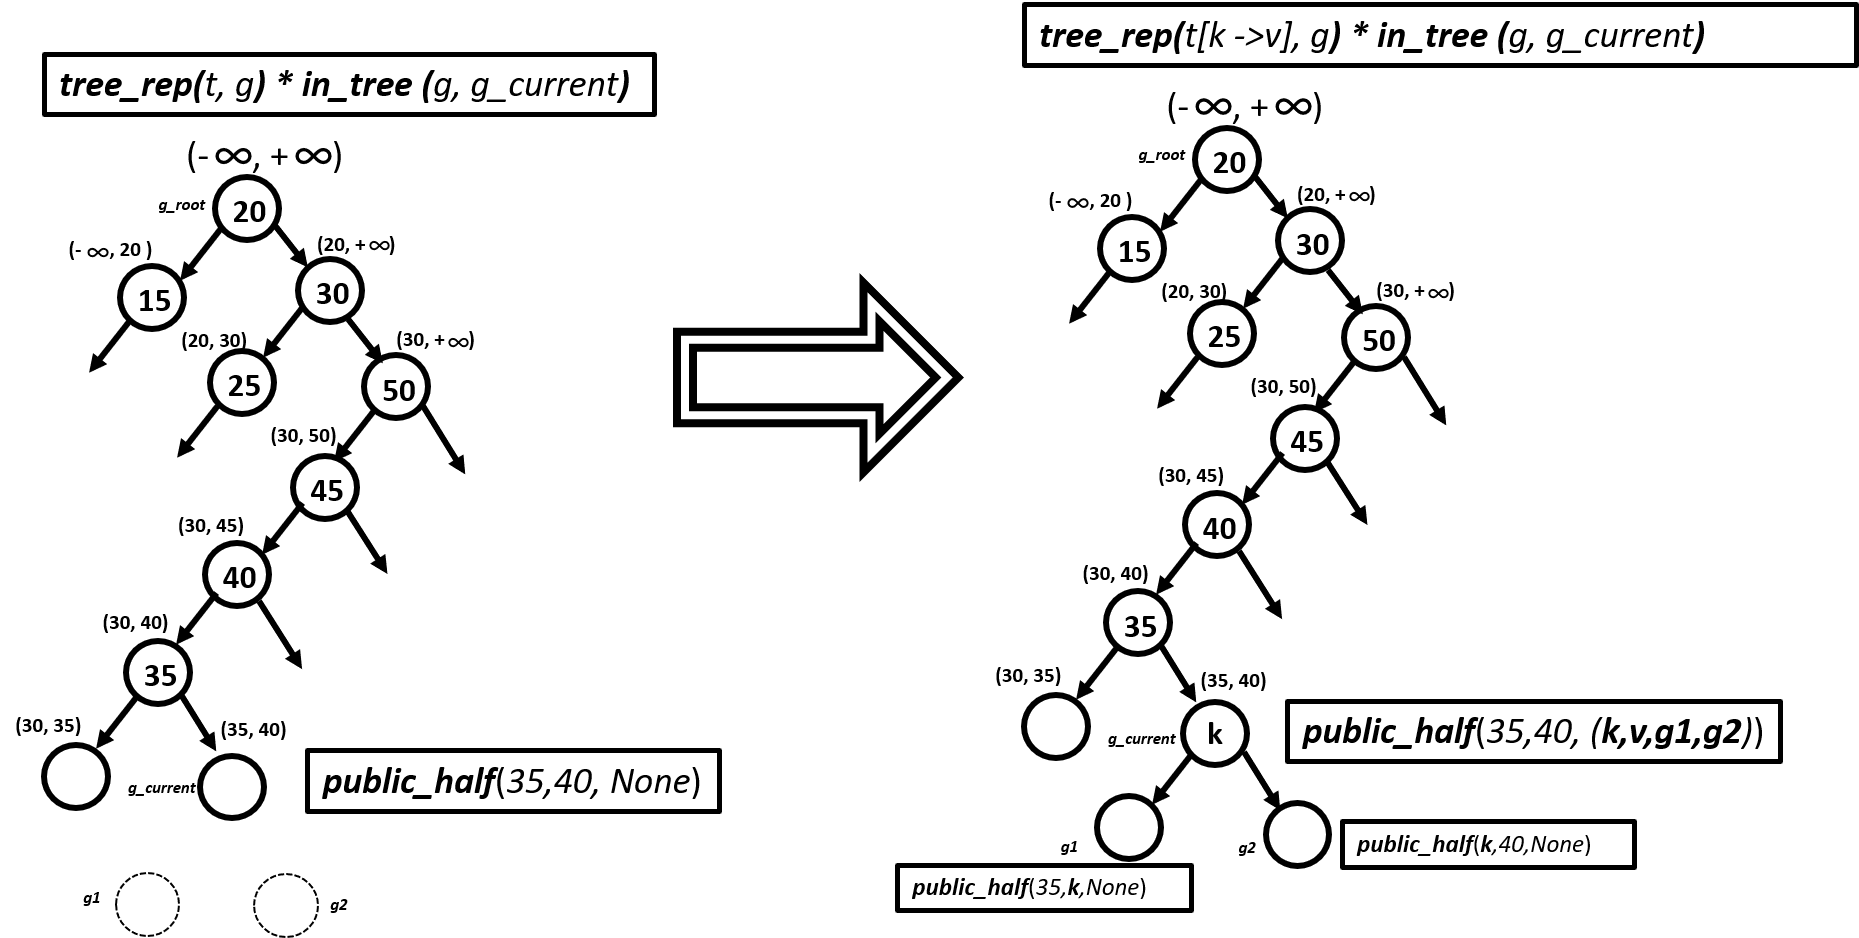
\includegraphics[width=150mm,scale=0.5]{FIG/extract_insert.png}
\caption{A visual depiction of the change in global state of BST during $\mathsf{insert(k,v)}$ operation }
\label{extract_insert}
\end{figure}
\begin{figure}[htb]
\centering
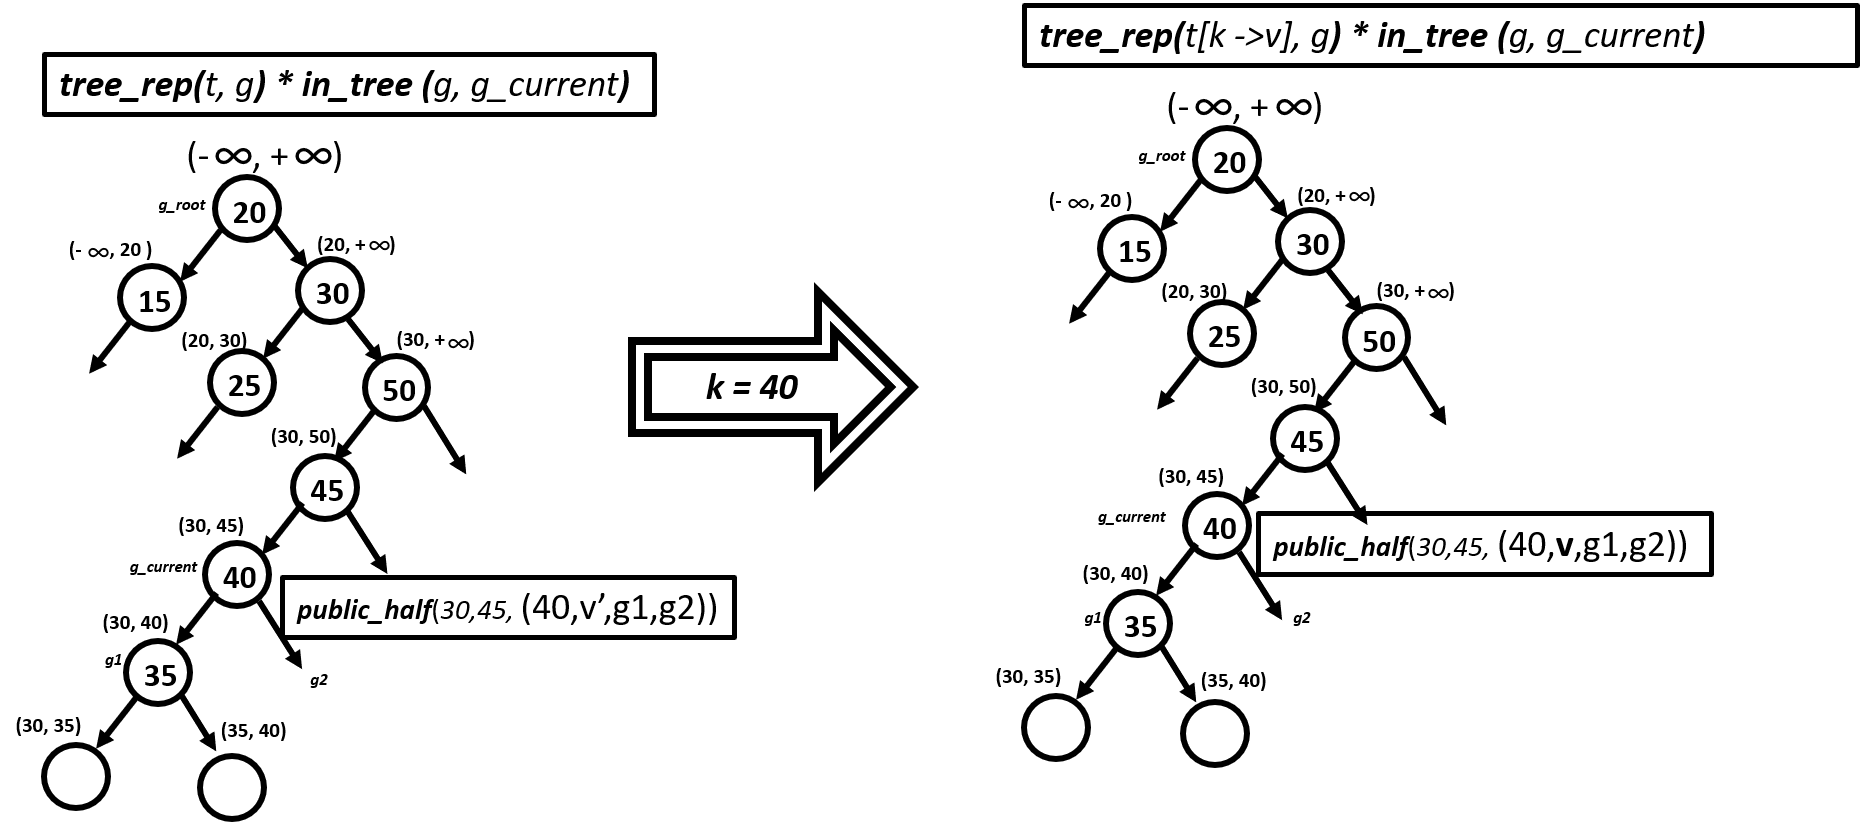
\includegraphics[width=150mm,scale=0.5]{FIG/extract_insert_2.png}
\caption{A visual depiction of the change in global state of BST during $\mathsf{insert(k,v)}$ operation, where key $k$ already exists in the tree $t$ }
\label{extract_insert2}
\end{figure}
\begin{figure}[htp]
\begin{subfigure}[t]{1\textwidth}
 $$\left\{\begin{array}{l} \nodeboxrep(b,g\_root)\ *\ \mathsf{atomic\_shift}(P_p,E_i,E_o,Q_p,Q)\end{array}\right\}$$
 \vspace*{-20pt}
\begin{lstlisting}[language = C,numbers = none]
insert(treebox t, int x, void *value)
  tree_t *tgt = *t;
  acquire(tgt->lock)
 \end{lstlisting}  
 $$\left\{\begin{array}{l} \ghost{\mathsf{my\_half}((-\infty,+\infty),info)}{g\_root}\ *\ R\ b\ *\ \mathsf{lock\_inv}(lock,lsh2,R')\ *\ \\
 \nodeboxrep(b,g\_root)\ *\ \mathsf{atomic\_shift}(P_p,E_i,E_o,Q_p,Q)\end{array}\right\} \Rrightarrow \left\{\begin{array}{l} insert\_inv \end{array}\right\}$$ 
  \begin{lstlisting}[language = C,numbers = none]
  for(;;) {
       \end{lstlisting}   
   $$\left\{\begin{array}{l} insert\_inv \end{array}\right\} \triangleq \left\{\begin{array}{l}(x\in range)\land \ghost{\mathsf{my\_half}(range,info)}{g\_current}*\ R\ np\ \\*\mathsf{lock\_inv}(lock,lsh2,R')\ *\ \nodeboxrep(b,g\_root)\ *\ \mathsf{atomic\_shift}(P_p,E_i,E_o,Q_p,Q)\end{array}\right\}$$
      \begin{lstlisting}[language = C,numbers = none]
    p = tgt->t;
    if (p==NULL)
      tree_t *p1, *p2 = malloc();
      p = malloc(); tgt->t = p;
      p->key=x; p->value=value; p->left=p1; p->right=p2;
           \end{lstlisting} 
  $$\left\{\begin{array}{l} \ghost{\mathsf{own}\ (a1)}{g1}\ *\ \ghost{\mathsf{own}\ (a2)}{g2}\ *\ \ghost{\mathsf{my\_half}(range,None)}{g\_current}*\ R\ np\ \\*\mathsf{lock\_inv}(lock,lsh2,R')\ *\ \nodeboxrep(b,g\_root)\ *\ \mathsf{atomic\_shift}(P_p,E_i,E_o,Q_p,Q)\end{array}\right\} \Rrightarrow{\textbf{sync\_commit}}$$
$$\left\{\begin{array}{l} \ghost{\mathsf{my\_half}(range,None)}{g\_current}*\ R\ np\ *\mathsf{lock\_inv}(lock,lsh2,R')\ *\ \nodeboxrep(b,g\_root)\ *\ Q\end{array}\right\}$$
 \vspace*{-10pt}
        \begin{lstlisting}[language = C,numbers = none]
      release2(l);
         \end{lstlisting}
       $$\left\{\begin{array}{l} \nodeboxrep(b,g\_root)\ *\ Q\end{array}\right\}$$
        \vspace*{-10pt}
         \begin{lstlisting}[language = C,numbers = none]
      return;
     else 
        ....
       else 
      	p->value=value;
      	\end{lstlisting} 
$$\left\{\begin{array}{l} \ghost{\mathsf{my\_half}(range,None)}{g\_current}*\ R\ np\ *
\mathsf{lock\_inv}(lock,lsh2,R')\ *\ \\\nodeboxrep(b,g\_root)\ *\ \mathsf{atomic\_shift}(P_p,E_i,E_o,Q_p,Q)\end{array}\right\} \Rrightarrow{\textbf{sync\_commit}}$$
$$\left\{\begin{array}{l} \ghost{\mathsf{my\_half}(range,None)}{g\_current}*\ R\ np\ *\mathsf{lock\_inv}(lock,lsh2,R')\ *\ \nodeboxrep(b,g\_root)\ *\ Q\end{array}\right\}$$
         \vspace*{-10pt}
      	\begin{lstlisting}[language = C, numbers = none]
        release2(l);
        \end{lstlisting}
        $$\left\{\begin{array}{l}  \nodeboxrep(b,g\_root)\ *\ Q\end{array}\right\}$$
         \vspace*{-10pt}
        \begin{lstlisting}[language = C, numbers = none] 
      	return;
\end{lstlisting}
\end{subfigure}
\caption{The $\texttt{insert}$ function annotated with separation logic specification}
\label{insertproof}
\end{figure} 

\paragraph{Changing the Global State} describe ``extract lemmas'' here

\subsubsection{Lookup}

The code for the $\mathsf{lookup}$ method is shown in Figure
\ref{lookupproof}. It takes the location of the root pointer and a key
as the arguments. A thread spans the tree to find a given key using
hand-over-hand locking mechanism. Once a thread finds the key in the
tree, it gets the value associated with that key, releases the current
node's lock, and returns the value.
The atomic specification for $\mathsf{lookup}$ is
$$\forall t.\ \langle \nodeboxrep\ p\ |\ \treerep\ t\rangle\ \texttt{lookup}(p, k)\ \langle v.\ \nodeboxrep\ p\ |\ \treerep\ t \land \mathrm{lookup}\ t\ k = v\rangle$$
The \texttt{lookup} function should atomically look up the value of the key $k$ in the tree at $p$.

As before, the key to the verification is the invariant for the main loop:
\begin{align*} &\mathsf{lookup\_inv}(b, x, \mathit{g\_root}, \mathit{range},\mathit{info}) \triangleq\ \exists\ \mathit{lock},\ \mathit{g\_current},\ \mathit{np},\ (x\in \mathit{range})\ \land \ \ghost{\mathsf{my\_half}(\mathit{range},\mathit{info})}{\mathit{g\_current}}\\& *\ R\ np\ * \mathsf{lock\_inv}(\mathit{lock},\mathit{lsh2},R')\ *\ \nodeboxrep(b,\mathit{g\_root})\ *\ \mathsf{atomic\_shift} (P_p,E_i,E_o,Q_p,Q) \end{align*}
where $P_p$ and $Q_p$ are $\treerep(g\_root, t)$ and $(v =
M[k])\ \wedge\ \treerep(g\_root, t)$ respectively. The proof steps for
the $\texttt{lookup}$ verification are similar to the steps
used in $\texttt{insert}$ verification, with a few differences which we
discuss below.

Figure \ref{lookupproof} shows the $\mathsf{lookup}$ function
with separation logic annotations. The proof starts with
$\nodeboxrep$ and $\mathsf{atomic\_shift}$ assertions as the
precondition and follows the same approach as the $\mathsf{insert}$
proof for the verification of loop body. Once we find the target key
(the last $\mathsf{else}$ clause in the code), we need
to confirm that the value present in the tree corresponds with the value we would find if we looked up the key in the current abstract state. We accomplish this by opening the global
invariant encoded in the $\mathsf{atomic\_shift}$, and proving that
lookup satisfies the public postcondition $\mathsf{Q\_p}$ with the help
of the $\mathsf{sync\_commit\_same}$ lemma described in section
\ref{atomicity}. This is the linearization point of the
$\mathsf{lookup}$ operation and must be done before releasing the
current node's lock. When we move into the left or right sub-tree,
we need to establish $\mathsf{lookup\_inv}$ at the end of the $\mathsf{if}$
or $\mathsf{else\ if}$ clause. Here, we need to show that the key we
are searching for is still in the range of our new node, so we use
$\mathsf{sync\_rollback}$ to extract the bound of the left/right
node encoded as the ghost state in the public precondition
($\treerep(M, g, g\_root)$).

A critical difference from $\texttt{insert}$ is that the
$\texttt{lookup}$ method does not change the shape of the tree. With the
help of $\texttt{sync\_commit\_same}$, we need no longer the
heavyweight $\emph{extract}$ lemma but instead a simpler
$\emph{ramif}$ lemma to locate the current node in the global
invariants:
\begin{verbatim}
Lemma ghost_tree_rep_public_half_ramif: forall tg g_root r_root g_in,
Ensembles.In (find_ghost_set tg g_root) g_in -> ghost_tree_rep tg g_root r_root |-- 
EX r: node_info, !! (range_info_in_tree r r_root tg) && (public_half g_in r * 
(public_half g_in r -* ghost_tree_rep tg g_root r_root)).
\end{verbatim}

\begin{figure}[htp]
\begin{subfigure}[t]{1\textwidth}
 $$\left\{\begin{array}{l} \nodeboxrep(b,g\_root)\ *\ \mathsf{atomic\_shift}(P_p,E_i,E_o,Q_p,Q)\end{array}\right\}$$
\begin{lstlisting}[language = C,  numbers = none]
void *lookup (treebox t, int x) {
  struct tree *p; void *v;  struct tree_t *tgt;
  tgt = *t;  void *l = tgt->lock;
  acquire(l);  p = tgt->t;
 \end{lstlisting}  
 $$\left\{\begin{array}{l} \ghost{\mathsf{my\_half}((-\infty,+\infty),info)}{g\_root}\ *\ R\ b\ *\ \mathsf{lock\_inv}(l,lsh2,R')\ *\ \\
 \nodeboxrep(b,g\_root)\ *\ \mathsf{atomic\_shift}(P_p,E_i,E_o,Q_p,Q)\end{array}\right\} \Rrightarrow \left\{\begin{array}{l} lookup\_inv \end{array}\right\}$$ 
  \begin{lstlisting}[language = C, numbers = none]
    while (p!=NULL) {
       \end{lstlisting}   
   $$\left\{\begin{array}{l} lookup\_inv \end{array}\right\} \triangleq \left\{\begin{array}{l}(x\in range)\land \ghost{\mathsf{my\_half}(range,info)}{g\_current}*\ R\ np\ *\\\mathsf{lock\_inv}(lock,lsh2,R')\ *\ \nodeboxrep(b,g\_root)\ *\ \mathsf{atomic\_shift}(P_p,E_i,E_o,Q_p,Q)\end{array}\right\}$$
      \begin{lstlisting}[language = C,  numbers = none]
    if (x<y){
      tgt=p->left;
      ....
    }else if (y<x){
      tgt=p->right;
     ....
    }else {
    v = p->value;
           \end{lstlisting} 
  $$\left\{\begin{array}{l} \ghost{\mathsf{my\_half}(range,info)}{g\_current}*\ R\ np\ *\mathsf{lock\_inv}(lock,lsh2,R')\ *\ \\\nodeboxrep(b,g\_root)\ *\ \mathsf{atomic\_shift}(P_p,E_i,E_o,Q_p,Q)\end{array}\right\} \Rrightarrow{\textbf{sync\_commit\_same}}$$
$$\left\{\begin{array}{l} \ghost{\mathsf{my\_half}(range,info)}{g\_current}*\ R\ np\ *\mathsf{lock\_inv}(lock,lsh2,R')\ *\ \nodeboxrep(b,g\_root)\ *\ Q\end{array}\right\}$$
        \begin{lstlisting}[language = C,  numbers = none]
      release2(l);
         \end{lstlisting}
       $$\left\{\begin{array}{l} \nodeboxrep(b,g\_root)\ *\ Q\end{array}\right\}$$
         \begin{lstlisting}[language = C, numbers = none]
       return v;} }
  release2(l);  return NULL;  }
 \end{lstlisting} 
\end{subfigure}
\caption{The $\texttt{lookup}$ function annotated with separation logic specification}
\label{lookupproof}
\end{figure} 

\subsection{Delete}

The code for the delete method is shown in ??. It takes the location of the root pointer
and a key as the arguments. A thread traverses the tree using hand-over-hand locking,
until the thread finds the key to be deleted. To remove the key, the tree is changed 
through an operation called pushdown left such that the node to be deleted points to an empty leaf
right child. To achieve that, the thread sets the right child's left child as the 
new right child of the to-be-deleted node and moves the right child's right child as 
the new parent of the to-be-deleted node. This operation is repeated until the right
child of the to-be-deleted node is an empty leaf node. Then, the thread will delete
the node and set the delete node's parent pointer to the left child of the deleted node.

The atomic specification for delete method can be written as follows:
$$\forall t.\ \langle \nodeboxrep(p,g,g\_root)\ |\ \treerep(t,g)\rangle $$ 
$$\texttt{delete}(p,k)$$
$$\langle \nodeboxrep(p,g,g\_root)\ |\ \treerep(\texttt{delete}(t, k),g)\rangle $$

The delete method is unique compared to insert and lookup because the pushdown left 
operation can change the \textit{public} half range of more than one nodes. In addition,
the pushdown left operation is one of the main reasons why the ghost tree of the binary
search tree is not just a ``copy" of the pure tree: the functional model of pushdown\_left
is unable to account for the change of deleted node's parent's pointer from pointing
at the deleted node the to the deleted node's right child.



\usetikzlibrary{positioning}

\forestset{
   lab/.style={
        label={[anchor=west, scale=0.75] north east:#1},
    },
}
\begin{forest}
for tree={
    grow=south,
    circle, draw, minimum size=3ex, inner sep=1pt,
    s sep=3mm
        }
    % my label/.style={
        % label={[anchor=south west] north east:#1},
    % },
    [, phantom, for children={fit=band}, s sep+=20mm,
         before drawing tree={%
          tikz+={%
            \node (a) [inner sep=0pt, fit=(!1) (!1L) (!1F)] {};
            \node (b) [inner sep=0pt, fit=(!l) (!lL) (!lF)] {};
            \node [anchor=center] at ($(a.east)!1/2!(b.west)$) {$\longrightarrow\quad$};
          },
        },
        [ 30, tikz={\node[right=0pt of .north east, scale=0.75]  {$(-\infty,\infty)$};}
            [25, tikz={\node[left=0pt of .north west, scale=0.75]  {$(-\infty,30)$};}]
            [75, tikz={\node[right=0pt of .north east, scale=0.75]  {$(30,\infty)$};}
                [40, tikz={\node[left=0pt of .north west, scale=0.75]  {$(30,75)$};}
                    [35, tikz={\node[left=0pt of .north west, scale=0.75]  {$(30,40)$};}]
                    [55, tikz={\node[right=0pt of .north east, scale=0.75]  {$(40,75)$};}
                        [50, tikz={\node[left=0pt of .north west, scale=0.75]  {$(40,55)$};}]
                        [60, tikz={\node[right=0pt of .north east, scale=0.75]  {$(55,75)$};}]
                    ]
                ]
                [80, tikz={\node[right=0pt of .north east, scale=0.75]  {$(75,\infty)$};}]
            ]
        ]
        [ 30, tikz={\node[right=0pt of .north east, scale=0.75]  {$(-\infty,\infty)$};}
            [25, tikz={\node[left=0pt of .north west, scale=0.75]  {$(-\infty,30)$};}]
            [75, tikz={\node[right=0pt of .north east, scale=0.75]  {$(30,\infty)$};}
                [55, tikz={\node[left=0pt of .north west, scale=0.75]  {$(30,75)$};}
                    [40, tikz={\node[left=0pt of .north west, scale=0.75]  {$(30,55)$};}
                        [35, tikz={\node[left=0pt of .north west, scale=0.75]  {$(40,35)$};}]
                        [50, tikz={\node[right=0pt of .north east, scale=0.75]  {$(40,55)$};}]
                    ]
                    [60, tikz={\node[right=0pt of .north east, scale=0.75]  {$(55,75)$};}]
                ]
                [80, tikz={\node[right=0pt of .north east, scale=0.75]  {$(75,\infty)$};}]
            ]
        ]
        [ 30, tikz={\node[right=0pt of .north east, scale=0.75]  {$(-\infty,\infty)$};}
            [25, tikz={\node[left=0pt of .north west, scale=0.75]  {$(-\infty,30)$};}]
            [75, tikz={\node[right=0pt of .north east, scale=0.75]  {$(30,\infty)$};}
                [55, tikz={\node[left=0pt of .north west, scale=0.75]  {$(30,75)$};}
                    [50, tikz={\node[left=0pt of .north west, scale=0.75]  {$(30,55)$};}
                        [40, tikz={\node[left=0pt of .north west, scale=0.75]  {$(30,50)$};}
                            [35, tikz={\node[left=0pt of .north west, scale=0.75]  {$(30,35)$};}]
                            [,no edge, draw=none]
                        ]
                        [,no edge, draw=none]
                    ]
                    [60, tikz={\node[right=0pt of .north east, scale=0.75]  {$(55,75)$};}]
                ]
                [80, tikz={\node[right=0pt of .north east, scale=0.75]  {$(75,\infty)$};}]
            ]
        ]
        [ 30, tikz={\node[right=0pt of .north east, scale=0.75]  {$(-\infty,\infty)$};}
            [25, tikz={\node[left=0pt of .north west, scale=0.75]  {$(-\infty,30)$};}]
            [75, tikz={\node[right=0pt of .north east, scale=0.75]  {$(30,\infty)$};}
                [55, tikz={\node[left=0pt of .north west, scale=0.75]  {$(30,75)$};}
                    [50, tikz={\node[left=0pt of .north west, scale=0.75]  {$(30,55)$};}
                        [35, tikz={\node[left=0pt of .north west, scale=0.75]  {$(30,35)$};}]
                        [,no edge, draw=none]
                    ]
                    [60, tikz={\node[right=0pt of .north east, scale=0.75]  {$(55,75)$};}]
                ]
                [80, tikz={\node[right=0pt of .north east, scale=0.75]  {$(75,\infty)$};}]
            ]
        ]
    ]
\end{forest}

\subsubsection{delete}

Similar with insert, delete starts by acquiring the root node lock, so that the thread
can access the information inside the lock invariant of the root node. Then, we prove
the while loop by showing that the precondition satisfies delete\_inv and the 
loop body preserves the loop invariant. The first two cases are similar to insert and
lookup in which the thread finds the target node, traversing by hand-over-hand locking.
Once the target node is located, the thread will call pushdown\_left and return after.
Using the specification of pushdown\_left, we show that the post-condition of 
pushdown\_left implies the loop invariant. Note that before going into pushdown\_left,
the thread is holding the lock to the target node and will return to the delete
method without holding any.

\subsubsection{pushdown\_left}

The proof to pushdown\_left is the key step of proving the delete method. 
First, we show that the precondition of pushdown\_left satisfies the precondition
of the loop invariant, which includes the assertion that the thread is holding the 
lock to the deleted node (i.e. the information inside the lock invariant is accessible)
and an atomic\_shift. Then, the thread accesses that information to acquire a second 
lock to the right child of the deleted node. Due to the hand-over-hand locking 
mechanism this will not cause a deadlock since the thread has already acquired the 
lock to the deleted node. Next, we prove that the action of deleting the node,
with sync\_commit by opening the global invariant and removing the relevant 
ghost names (the target node and its right sentinel node), satisfies the loop
invariant and the postcondition of pushdown\_left.

The second part of pushdown\_left is proving that the turn\_left operation satisfies
the loop invariant. Using a variant of the sync\_rollback rule, we show that the 
turn\_left operation preserves the BST, apart from changes in the ranges of two nodes,
the target node and its right child, and information about the nodes in those two nodes.
To satisfy the structure of the ranges, we only need to prove that the new range for
the target node is encompasses the old range of both nodes. This will imply that
the range of the target node's old parent includes the target node's right child 
new range as the right child becomes the new parent (and the old parent points to 
the right child).

One key step of the proof is proving that two ghost trees are equivalent if the union
of its ghost nodes are equal and the ghost tree is sorted. This allows the global invariant
to be preserved during the turn\_left operation in which no nodes were actually changed
except for the structure of the tree.


\section{Lock-Free BST}
We want to prove that a lock-free BST implementation satisfies the same specification as our hand-over-hand implementation. Unfortunately, provably-correct deletion in a lock-free setting is a research topic in itself (cite?), so we begin with a lock-free BST that only supports insert and lookup. Once again, we want to prove
\begin{mathpar}
\forall t.\ \langle \nodeboxrep\ p\ |\ \treerep\ t\rangle\ \texttt{insert}(p, k, v)\ \langle \nodeboxrep\ p\ |\ \treerep\ (\mathrm{insert}\ t\ k\ v)\rangle

\forall t.\ \langle \nodeboxrep\ p\ |\ \treerep\ t\rangle\ \texttt{lookup}(p, k)\ \langle v.\ \nodeboxrep\ p\ |\ \treerep\ t \land \mathrm{lookup}\ t\ k = v\rangle
\end{mathpar}
though the precise definitions of $\nodeboxrep$ and $\treerep$ will differ. %something about how the fact that the specs are the same really comes across to a client -- and should we prove a client?

\section{Using the Specifications}
client and client proofs

\section{Related Work}
\label{related}
Our work is based on the concurrent separation logic of VST in the style of Iris \cite{higherorderghoststate} and the logical atomicity from TaDA logic  \cite{tada}. The notion of the \emph{lower} and \emph{upper} bound is taken from the flow interface paper \cite{krishna2017flow}. Our main technical contributions are the verification of two different implementation of binary search tree (using fine-grained locking and lock-free technique) with respect to the same abstract specification, and first c-level mechanized verification of concurrent search-based data structure (i.e. BST). Most of the other concurrent separation logic (CSL)-based verification works are on toy languages, while VST lets us use the same logic on real C programs. 

Gotsman and Yang \cite{gotsman} is one of the earliest work on concurrent separation logic. They introduced the program logic to reason locally about the heap-manipulating program with the notion of dynamic ownership of heap parts by unbounded number of locks and threads, and shown the verification of singly-linked list with fine-grained locking. Xiong et al. \cite{Xiong2017Abstract} have demonstrated the verification of ConcurrentSkipListMap from java.util.concurrent library using the recent advances in fine-grained concurrency reasoning. Their work is mainly based on the abstract atomicity from TaDa logic, and give two modular specifications for concurrent maps: one specification focus on the entire map structure which is suitable for verifying implementation, and another specification focus on the key-value pairs which appropriate for verifying clients. We use the same idea of atomicity (though implemented in Iris) in our work. 

Krishna et al. \cite{krishna2017flow} have presented the proof technique for concurrent search structure templates based on the flow framework and the Iris separation logic, and verified the implementation of concurrent B-tree, hash tables, and linked lists based on the templates. Their work is closely related to our work; we took some inspiration from them in building our ghost state. But, their proofs are on a toy language rather than real C code.

\section{Conclusion}
\label{conclusion}

%% Bibliography
\bibliography{sources}
\end{document}
